\chapter{Introducción}

%\section{Historia de los métodos numéricos}

\section{Razones de su aplicación en la Ingeniería}
La matemática y la física nos permite describir fenómenos de la naturaleza a través de modelos. El planteamiento de dichos modelos
generalmente resulta en un problema matemático. 

Por ejemplo, imagine que se desea calcular el área debajo de un puente y supongamos que el área formada por el puente no es una figura simple. 
Este cálculo podría hacerse a través de una integral, para ello es necesario obtener una función que modele la parte inferior del puente y plantear
la integral definida. Ahora al resolver la integral se podría obtener dicha área, y la calidad de la aproximación dependerá de lo preciso que sea
el modelo generado para el bajo-puente.

Por ello si se desea mejorar el cálculo habría que mejorar el modelo. Ahora si el modelo resulta una función complicada, ¿qué ocurriría si la integral
no se puede resolver analíticamente?. Debe ser claro que el área existe a pesar de que la integral pueda o no resolverse analíticamente. 

Para fines prácticos, nos interesa el resultado más no si éste se obtuvo de manera analítica o no. Es en este escenario donde los métodos numéricos
resultan muy útiles. 

\begin{verse}
\textit{Los métodos numéricos nos permiten obtener una aproximación a la solución de un problema matemático, más no resolverlo.} 
\end{verse}

¿Cuál es la diferencia entre resolver y aproximar a la solución de un problema matemático?. Resolver un problema matemático consiste en encontrar
una expresión, un teorema, o una regla para ese problema; es una solución que incluye una generalización para una familia de problemas semejantes.
Una aproximación a la solución es un valor numérico para un problema específico de esa familia.

El único precio que se paga por utilizar un método numérico es que las aproximaciones incluyen un error por su mera naturaleza.


\section{Conceptos básicos}

\begin{description}
	\item[Cifra significativa. ] El concepto de cifras o dígitos significativos se ha desarrollado para designar formalmente la confiabilidad de 
		un valor numérico. Las cifras significativas de un numero son aquellas que pueden utilizarse de forma confiable. Se trata del numero de dígitos 
		que se ofrecen con certeza, más uno estimado. Por ejemplo, el velocímetro y el odómetro de un automóvil mostrado en la figura \ref{fig:odometro}.
		\begin{figure}[H]
			\centering
			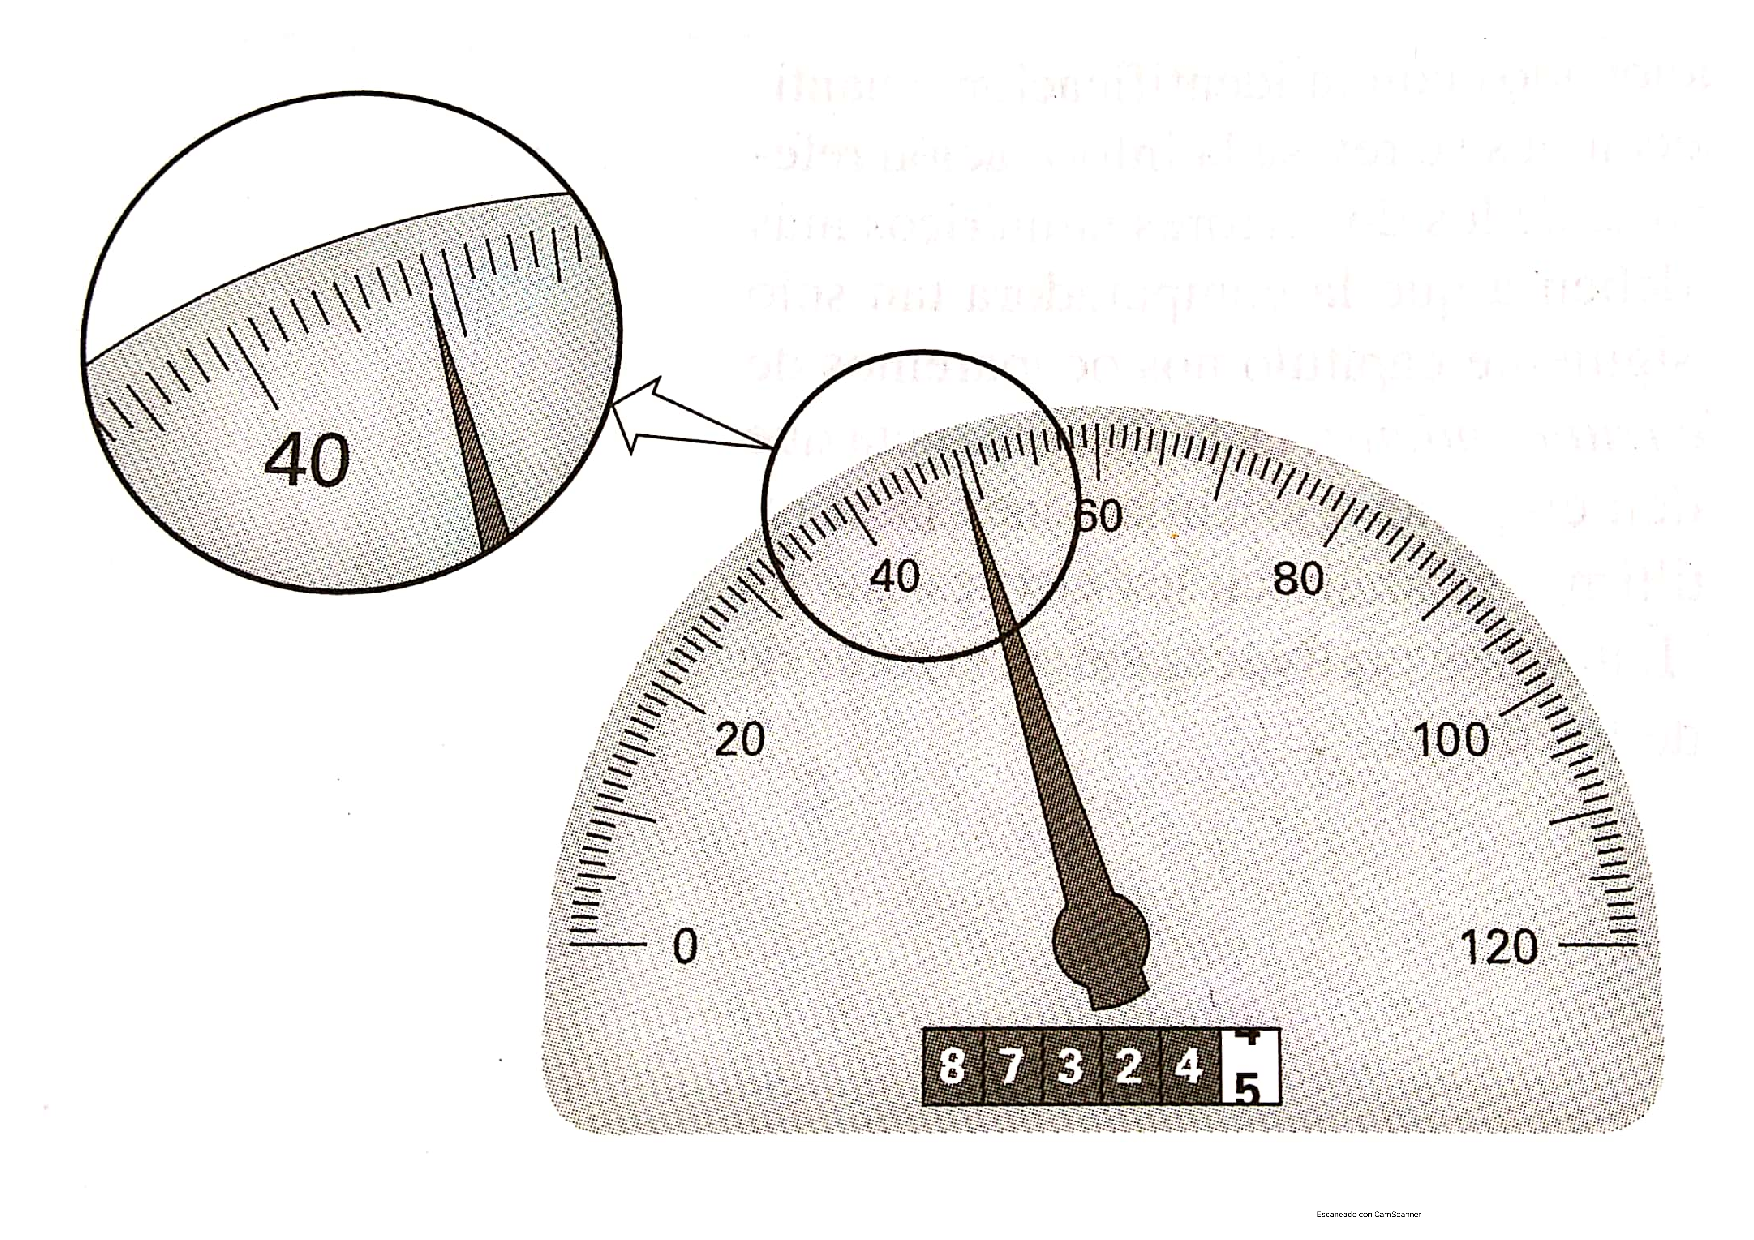
\includegraphics[scale=0.25]{img/odometro.pdf}
			\caption{El odómetro y velocímetro de un automóvil ejemplifican el concepto de cifras significativas.}
			\label{fig:odometro}
		\end{figure}
	\item[Exactitud e incertidumbre. ] Se refiere a que tan cercano está el valor calculado o medido del valor verdadero.
	\item[Precisión y error. ] Se refiere a que tan cercanos se encuentran, unos de otros, diversos valores calculados o medidos.
\end{description}

Estos conceptos se ilustran gráficamente utilizando la analogía con una diana en la práctica de tiro. Los agujeros en cada blanco de la figura 
\ref{fig:exactitudPrecision} se consideran como las predicciones con una técnica numérica; mientras que el centro del blanco representa la verdad. 

La \textit{inexactitud} (conocida también como \textit{sesgo}) se define como una desviación sistemática del valor verdadero. Por lo tanto, aunque 
los disparos en la figura \ref{fig:exactitudPrecision}c están más juntos que los de la figura \ref{fig:exactitudPrecision}a, los dos casos son
igualmente inexactos, ya que ambos se centran en la esquina superior izquierda del blanco. 

La \textit{imprecisión} (también llamada \textit{incertidumbre}),
por otro lado, se refiere a la magnitud en la dispersión de los disparos. Por consiguiente, aunque las figuras \ref{fig:exactitudPrecision}b y 
\ref{fig:exactitudPrecision}d son igualmente exactas (esto es, igualmente centradas con respecto al blanco), la última es más precisa pues los 
disparos están agrupados en forma más compacta.

\begin{figure}[H]
	\centering
	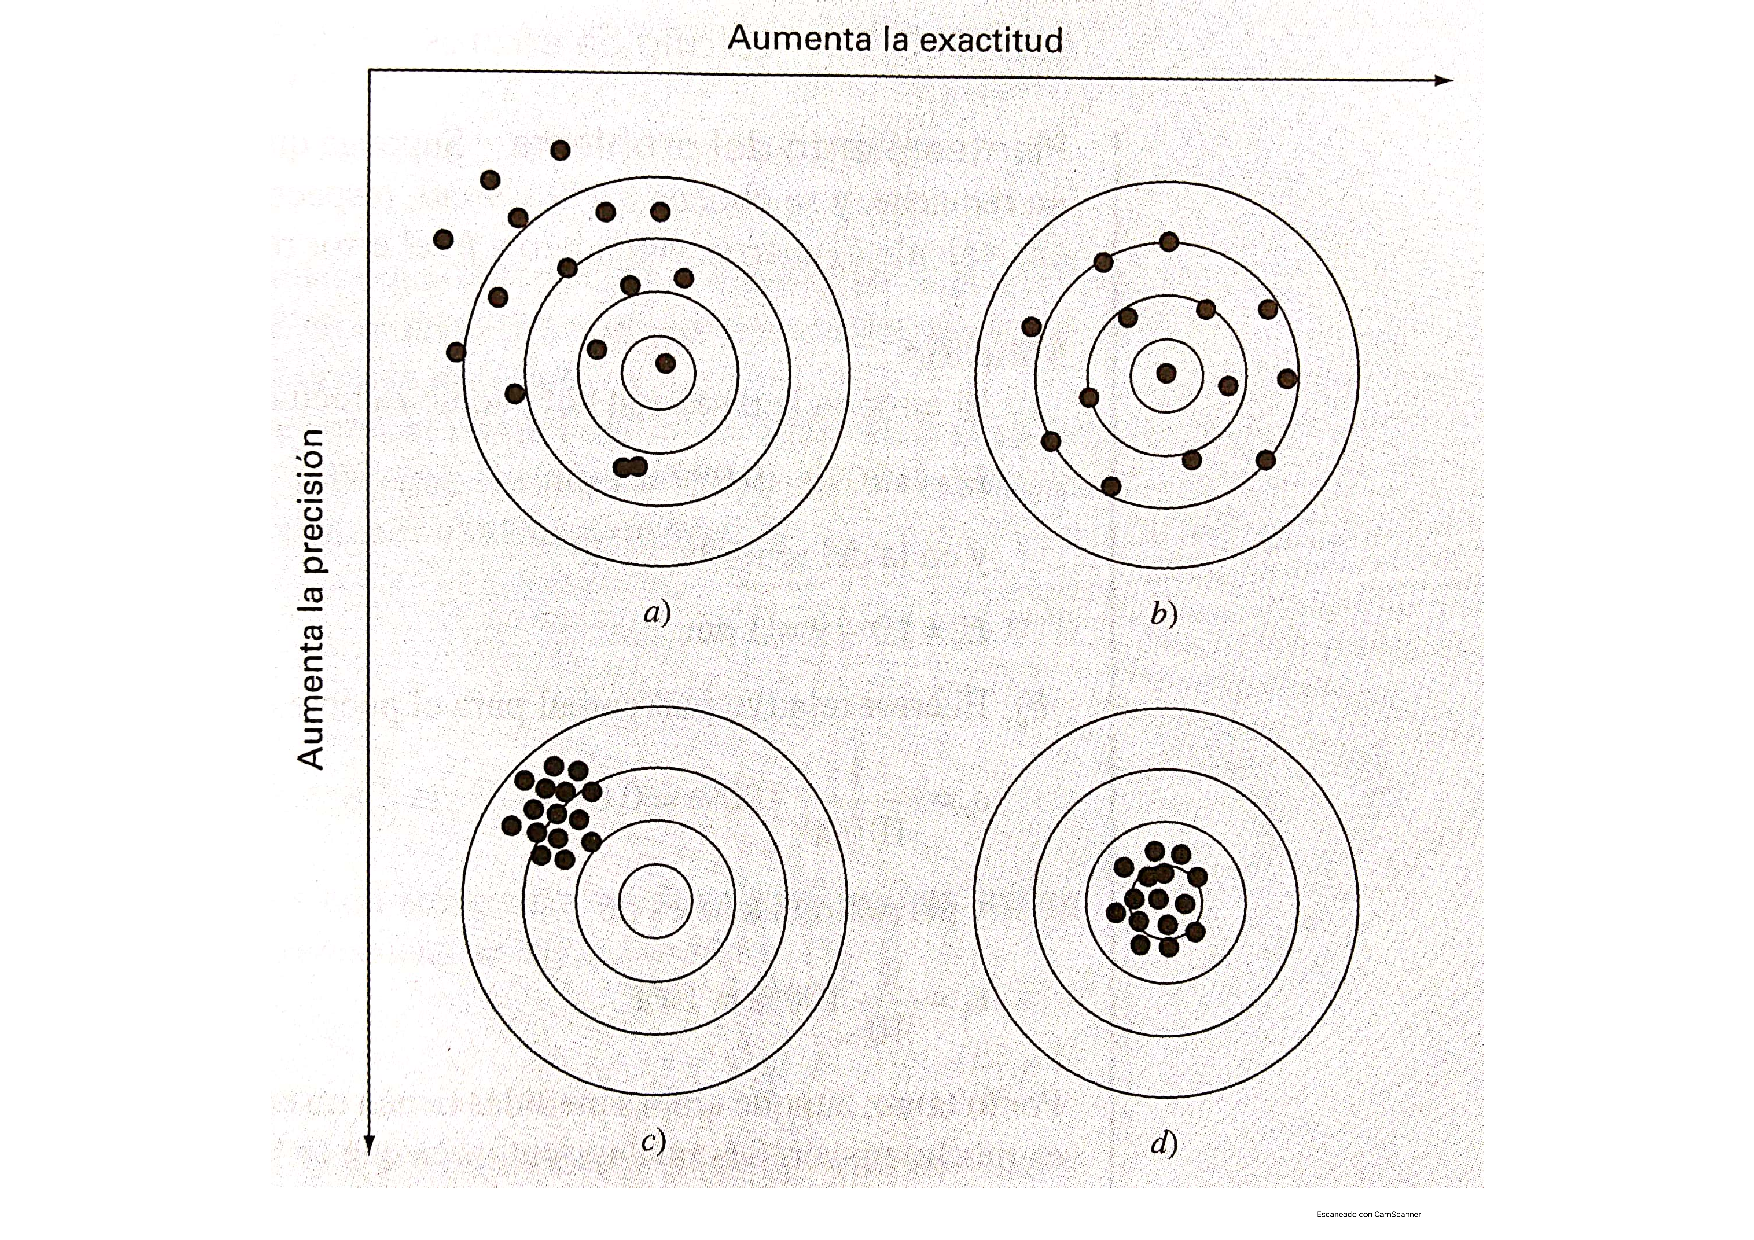
\includegraphics[scale=0.4]{img/exactitudPrecision.pdf}
	\caption{Exactitud y precisión}
 	\label{fig:exactitudPrecision}
\end{figure}


\section{Tipos de errores}
Los métodos numéricos permiten encontrar aproximaciones a la solución de diversos problemas matemáticos. Sin embargo, el hecho de utilizar estos métodos 
introduce errores en la aproximación. A continuación se describen algunos de los errores que ocurren.

\subsection{Error absoluto}

Una aproximación, por definición, es un valor cercano a la solución del problema, la cuál llamaremos absoluta. De esta forma, la diferencia entre la solución
absoluta y la aproximación a ella la llamaremos error absoluto. Es decir, si sumamos la aproximación y el error absoluto se obtiene la solución absoluta.\\

Este error absoluto es inevitable en los métodos numéricos y su estimación es compleja, incluso más que el método numérico que determina la aproximación. Por 
esta razón es que el cálculo del error absoluto resulta impractico y se opta por utilizar estrategias en la obtención de la aproximación para minimizar este 
error.

\subsection{Error de redondeo y truncamiento}

Utilizar una herramienta digital para el cómputo numérico tiene muchas ventajas pero también desventajas. Entre sus ventajas más relevantes se encuentra el 
hecho de que los sistemas digitales permiten la realización de cálculos aritméticos rápidamente, lo cual es muy conveniente para los métodos iterativos. 
Una desventaja relevante de los sistemas digitales es el hecho de que cuentan con una capacidad finita de memoria, aún y cuando esta capacidad de memoria se 
incrementa día a día, sigue siendo finita.\\ 

Tomemos un ejemplo específico, sea el número
\[ \dfrac{1}{3} = 0.33333\dots, \ \]
este número tiene un número infinito de cifras, un ligero cambio en alguna de esas cifras (por pequeña que sea) implica que el número ya no sea el mismo. 
Si el número no se escribe en su forma racional, será necesario emplear el número infinito de cifras para realizar un trato \textit{preciso} del número. \\

Cuando este número se almacena en la memoria de un sistema digital, no podrán almacenarse todas las cifras de este número dado que la memoria es finita. 
Esto significa que el número será almacenado solamente con una cantidad limitada de cifras significativas, lo que significa que ya no será estrictamente 
el mismo número. Esto se llama \textbf{truncamiento}.
Por otro lado, cuando se realizan operaciones con números truncados podrían obtenerse resultados imprecisos, esto llama \textbf{error de truncamiento}.\\

Vayamos a un ejemplo. En este ejemplo utilizaremos nuevamente el número $\frac{1}{3}$ y realizaremos operaciones aritméticas con el para mostrar el 
error de truncamiento. Supongamos que el sistema digital solo es capaz de almacenar 6 cifras significativas.

\begin{table}[H]
	\centering
	\begin{tabular}{cc}
		\toprule
		\textbf{Aritmética convencional} & \textbf{Aritmética digital con truncamiento}\\
		\midrule
		$\frac{1}{3}$ & $0.333333$\\
		$3\times\frac{1}{3}$ & $3\times 0.333333$\\
		$1$ & $0.999999$	\\	
		\bottomrule
	\end{tabular}
	\caption{Ejemplo del error de truncamiento}
	\label{table:errorTruncamiento}
\end{table}

En la tabla \ref{table:errorTruncamiento} se muestra la diferencia entre la aritmética convencional y digital, con el número completo y el número truncado. 
En el resultado es evidente que  formalmente $1\not= 0.999999$, y aunque se tenga un mayor número de cifras en el número digital siempre serán desiguales 
los resultados. En un caso práctico se dice que $1\approx 0.999999$, asumiendo que la diferencia es resultado del error de truncamiento.\\

El redondeo es similar al de truncamiento, solo que este ocurre cuando se ajusta el resultado de la operación a su inmediato superior o inferior, aquel que se
encuentre más cerca. El redondeo es una forma en la que los sistemas digitales pueden compensar el error de truncamiento, en el ejemplo mostrado en la tabla 
\ref{table:errorTruncamiento} lo compensaría apropiadamente, pero en otros casos no. Cuando el redondeo no compensa el truncamiento y en su lugar aleja al 
número de su valor absoluto, se dice que ocurre un \textbf{error de redondeo}. \\

Veamos un ejemplo en el que ocurre el error de redondeo y afecta al resultado obtienido en la operación. Considere los siguientes números y qu se hará
un redondeo de 6 cifras significativas del número.

\begin{table}[H]
	\centering
	\begin{tabular}{ccc}
		\toprule
		\textbf{Número racional} & \textbf{Valor numérico} & \textbf{Valor numérico redondeado}\\
		\midrule
		$2/7$ & $0.2857142857$ & $0.285710$\\
		$5/7$ & $0.7142857143$ & $0.714285$	\\
		\bottomrule
	\end{tabular}
	\caption{Valor numérico redondeado}
	\label{table:errorRedondeo}
\end{table}

Al realizar la suma de los números se obtiene un resultado inesperado e incorrecto debido al error de redondeo.

\begin{table}[H]
	\centering
	\begin{tabular}{cc}
		\toprule
		\textbf{Aritmética convencional} & \textbf{Aritmética digital con redondeo}\\
		\midrule
		$\frac{2}{7}$ & $0.285710$\\
		+ & + \\
		$\frac{5}{7}$ & $0.714285$\\
		= & = \\
		$1$ & $0.999995$		
	\end{tabular}
	\caption{Ejemplo del error de redondeo}
	\label{table:errorTruncamiento}
\end{table}

Por último, cabe mencionar que estos errores pueden combinarse en las operaciones aritméticas digitales, la gravedad de sus efectos dependerán completamente 
de los números y las operaciones que se hagan con ellos.

\section{Uso de herramientas computacionales}
Los métodos numéricos constituyen técnicas mediante las cuales es posible formular problemas matemáticos, de tal forma que puedan resolverse
utilizando operaciones aritméticas. Aunque existen muchos tipos de métodos numéricos, éstos comparten una característica común: invariablemente
requieren de un buen número de tediosos cálculos aritméticos. No es raro que con el desarrollo de computadoras digitales eficientes y rápidas, 
el papel de los métodos numéricos en la solución de problemas en ingeniería haya aumentado de forma considerable en los últimos años.

Antes del uso de la computadora se gastaba bastante energía en la técnica misma de solución, en lugar de usarla en la definición del problema
y su interpretación. Esta situación desafortunada se debía al tiempo y trabajo monótono que se requería para obtener resultados numéricos con
técnicas que no utilizaban la computadora. 

En la actualidad, las computadoras y los métodos numéricos ofrecen una alternativa para los cálculos complicados. Al usar el poder del cómputo
se obtienen soluciones directamente, de esta manera se pueden aproximar los cálculos sin tener que recurrir a consideraciones de simplificación
o a técnicas muy lentas. Aunque las soluciones analíticas aún son muy valiosas, tanto para resolver problemas como para brindar una mayor
comprensión, los métodos numéricos representan opciones que aumentan, en forma considerable, la capacidad de enfrentar y resolver los problemas;
como resultado, se dispone de más tiempo para aprovechar las habilidades creativas personales. En consecuencia, es posible dar más importancia
a la formulación de un problema y a la interpretación de la solución.

Para la gran mayoría de los métodos numéricos, es posible describir su desarrollo y representarlo mediante un algoritmo. En este sentido, 
resulta en extremo práctico utilizar una computadora para delegarle los cálculos que sean necesarios para encontrar una aproximación. 
Es muy importante recalcar que la computadora o bien el software que corre en ella, sólo son herramientas que ayudan al humano a resolver 
(o aproximar a la solución de) un problema.